\documentclass[10pt,twocolumn]{IEEEtran}
% arXiv preprint. Not the ICRA paper: this is the umbrella the two planned papers hang from.
% See OUTLINE.md for the claim discipline: it must NOT spend Paper 1's claim (detectability, E1-E3).
\IEEEoverridecommandlockouts
\usepackage[T1]{fontenc}
\usepackage[utf8]{inputenc}
\usepackage{amsmath,amssymb,graphicx,booktabs,siunitx,balance,array,tikz,xcolor}
\usetikzlibrary{arrows.meta,positioning}
\usepackage[hidelinks]{hyperref}
\sisetup{detect-weight=true,detect-family=true}
\newcommand{\asg}{ASG}
\newcommand{\efe}{\ensuremath{G}}
\newcommand{\nats}{nats}
\newcommand{\pdet}{\ensuremath{P(\mathrm{detect})}}
\newcommand{\todo}[1]{{\color{red}\textbf{[TODO: #1]}}}
\newcolumntype{P}[1]{>{\raggedright\arraybackslash}p{#1}}

\begin{document}

\title{Active Scene Graphs:\\a scene graph that acts to keep itself true}

% TODO(authors): confirm the author list and order; taken from the IWAI 2026 abstract.
\author{\IEEEauthorblockN{Pablo Bustos, No\'e Zapata, Pedro N\'u\~nez}\\
\IEEEauthorblockA{RoboLab, Universidad de Extremadura, C\'aceres, Spain}}

\maketitle

\begin{abstract}
A scene graph is usually a record: a data structure that perception fills and planning reads. This
paper proposes the \emph{Active Scene Graph} (\asg), a scene graph that acts to keep itself true.
Its nodes are concepts, each carrying a posterior and a precision; each concept publishes what the
robot could do to reduce its own uncertainty; the robot's body is itself one of these concepts and
calibrates itself through the same machinery; and a single controller ranks every published offer in
one currency, \nats, and executes it in real time over a distributed graph. We formulate this as
five requirements on a scene graph: that it be actionable, epistemically self-constructing,
concept-oriented, that it embed a self-calibrating model of the robot, and that it run in real time
across several processes. Taken individually, each of these has been met before. Our contribution is
to show that they are coupled, so that a system meeting them must meet them together, and to present
a system that does. We describe the underlying model, in which concept nodes carry posterior,
precision and existence, affordances are priced offers, and a single expected free energy governs both
representation and action, differing only by a task prior; the architecture that supports the
concurrency requirements, built on a replicated graph, a zero-copy media plane and two protocols
verified in TLA+; and an evaluation of the running parts in simulation and on two physical robots,
requirement by requirement. A ledger records what is designed, implemented and evaluated.
\end{abstract}

\section{Introduction}\label{sec:intro}

Three-dimensional scene graphs have become the representation of choice for robots that must reason
about places, objects and the relations between
them~\cite{armeni20193dscenegraphstructure,rosinol20203ddynamicscenegraphs,hughes2022hydra,gu2023conceptgraphsopenvocabulary3dscene}.
In all of these systems, however, the graph is a record. Perception writes nodes and edges, planning
reads them, and the graph itself neither knows how uncertain it is nor does anything about it. When
the record is wrong, nothing inside the representation notices; when it is incomplete, completing it
falls to something outside it, whether an exploration module following a frontier, a task planner
driven by a language model, or a person holding a joystick.

This paper describes a scene graph that is not a record but the thing that acts. In an
\emph{Active Scene Graph}, every node is a \emph{concept}: a belief with a mean, a covariance, a
precision and a log-odds of existence, maintained by the agent that owns it. Every concept publishes,
as nodes in the same graph, the actions the robot could take to reduce that concept's uncertainty,
each priced in \nats. The robot's own body is a concept in exactly this sense, and its kinematic and
extrinsic parameters are beliefs that the same machinery corrects online. A single controller ranks
every published offer, whatever its origin, under one expected free energy, and a task enters the
system as nothing more than a prior preference added to that functional. The layer that keeps the
representation true and the layer that pursues a goal are the same layer, distinguished by one term.

We develop this idea as five requirements (\S\ref{sec:req}). Each of them, taken on its own, has
been met by earlier work, and our contribution does not lie in any single one. It lies in the
observation that the requirements depend on one another. An actionable offer needs a calibrated
probability behind it; a calibrated probability needs a solved model of the robot; several
concurrent writers need ownership; ownership needs a transport that guarantees cleanup; bounded
bandwidth needs a graph that carries beliefs rather than pixels; and the robot model learns only
because acting is the experiment that teaches it. Satisfying the requirements one at a time
therefore does not compose into a system that satisfies them all, and each of these dependencies
surfaced, in our own system, as a concrete failure that was only resolved once the neighbouring
requirement was met.

The contributions are, first, the five requirements and the argument that couples them
(\S\ref{sec:req}); second, the model, in which concept nodes carry posterior, precision and existence,
affordances are priced offers, and one expected free energy serves both regimes
(\S\ref{sec:def}, \S\ref{sec:efe}); third, the robot as a concept that calibrates itself from the
corrections ordinary actions generate (\S\ref{sec:self}); fourth, an architecture that meets the
concurrency requirements, with two of its protocols verified in TLA+ (\S\ref{sec:arch}); fifth, an
evaluation of the running parts in simulation and on two physical robots, including a null result and
its explanation (\S\ref{sec:eval}); and finally a ledger of what is designed, implemented and
evaluated (Table~\ref{tab:ledger}).

The preprint grows out of two earlier pieces of our own work. An abstract at
IWAI~\cite{bustos2026active} introduced the actionable graph to an active-inference audience, with
viewpoints selected by a Fisher-information proxy, and the concept-first architecture
of~\cite{zapatacornejoConceptGuidedExplorationBuilding2025} built rooms and doors as cooperating
agents, but as a set of design intentions rather than a formalisation. What this paper adds to both is
the requirement set and its coupling, the single-currency pricing of offers, the self-calibrating
robot concept, and the evaluation.

\section{Five requirements, and why they are one}\label{sec:req}

Table~\ref{tab:req} states the requirements. Its second column gives, for each, the sentence the
paper commits to, phrased so that it could turn out to be false. The third column describes what a
system of the Hydra or ConceptGraphs class does instead, the fourth names the mechanism by which we
meet the requirement, and the last two give its status, using the ledger's three letters
(D~designed, I~implemented, E~evaluated), and the evidence behind it.

\begin{table*}[t]
\centering\small
\caption{The five requirements. D~designed, I~implemented, E~evaluated.}
\label{tab:req}
\setlength{\tabcolsep}{4pt}
\begin{tabular}{P{1.4cm}P{3.9cm}P{2.7cm}P{4.4cm}P{1.2cm}P{2.5cm}}
\toprule
\textbf{R} & \textbf{Falsifiable statement} & \textbf{Standard scene graph} & \textbf{Mechanism here} & \textbf{Status} & \textbf{Evidence} \\
\midrule
\textbf{R1} Actionable &
Every node carries executable offers whose preconditions are probabilities read from the graph, and one generic executor runs any of them without knowing the concept. &
Nodes are labels plus geometry; actions are planned outside the graph from a task specification. &
Affordance nodes under a \texttt{has\_intention} edge; epistemic offers (one per object) and pragmatic offers (named, preconditioned: approach, open, cross a door). Execution claim = epoch + an \texttt{executing} edge the consumer owns. &
protocol I+E; door offers I; task-level EFE D &
TLA+ model of the claim protocol; \S\ref{sec:eval:r1} \\
\addlinespace
\textbf{R2} Epistemic self-construction &
The graph's own posterior uncertainty is consumed: it gates publication and is priced into the offers the robot acts on. No hand thresholds in the belief pipeline. &
Uncertainty, if tracked, is stored; exploration is a frontier heuristic. &
Per-concept generative model with an adequacy target $\Sigma^\star$; next view from $\Delta H$ weighted by \pdet; existence as log-odds with absence weighted by \pdet\ and occlusion holding; a structural adoption judge for the room. &
I+E (objects, room); existence I &
Calibrated corner $\sigma$ on a physical robot; 50 synthetic rooms; 594 real layouts (null, \S\ref{sec:eval:r2}) \\
\addlinespace
\textbf{R3} Concept-oriented &
The graph is populated by independent concept agents, each owning one class of node under a normative lifecycle, and the fleet composes without a central planner. &
One monolithic mapper; classes are labels on one pipeline. &
Lifecycle contract (create, update, remove, history, ownership) with a per-agent conformance audit; ten concept agents plus meta-concepts and a long-term memory; an \texttt{owns} attribute ties node identity to agent identity. &
I+E &
Conformance audit; phantom births 130$\to$1 (\S\ref{sec:eval:r3}) \\
\addlinespace
\textbf{R4} Self-calibrating robot model &
The robot is a node like any other: its kinematic and extrinsic parameters are beliefs updated online from the localiser's own correction, and their precision propagates into every offer's price. &
The robot is a fixed URDF; calibration is offline. &
Robot frame tree as a concept; batch estimator over episodes; closed-loop camera extrinsics; wheel-odometry covariance injection; motion preintegration. &
I+E &
Extrinsic yaw recovery 0.984; boresight $+0.814^\circ$ applied (\S\ref{sec:eval:r4}) \\
\addlinespace
\textbf{R5} Real-time, distributed &
$N$ agents on $M$ machines share one graph with bounded latency; sensor streams bypass the graph; agents join and leave without corrupting it. &
A single process, or ROS topics with one map owner. &
CRDT graph; zero-copy media plane on a dedicated DDS domain; debounced presence protocol; ownership cleanup on graceful exit. &
I+E &
Stream lag 35$\to$9 ms; join/leave (\S\ref{sec:eval:r5}) \\
\bottomrule
\end{tabular}
\end{table*}

\subsection{The coupling argument}\label{sec:coupling}

A checklist can be satisfied one row at a time. The requirements above cannot, because of a set of
dependencies between them which we describe here and draw in Fig.~\ref{fig:coupling}. Each arrow
corresponds to something that went wrong in our own fleet and was resolved only by meeting the
requirement at the arrow's head.

\paragraph{Actionable needs calibrated, and calibrated needs a self-model} The price of an offer is
a log-probability, so the precondition of a pragmatic offer, such as the probability that a door is
open, is only worth acting on if the posterior behind it is calibrated. In our system that
calibration was reached only once the extrinsics of the robot's own sensors had been solved. A
boresight error of under a degree in one camera displaced every corner it observed by a few
centimetres, and it did so in a way that shrank the declared uncertainty rather than inflating it,
because the error was systematic and the precision estimate could only see what averaged away.

\paragraph{Epistemic self-construction needs ownership} When several agents write into a belief
pipeline, each must own what it writes. Before ownership was made explicit, two agents held different
values of ``the target'' of an offer, and neither could detect the disagreement, because the channel
between them returned a boolean rather than the pose being executed. The cure was an edge that the
consuming agent owns, carrying the target it is actually pursuing and an epoch that both sides can
compare: a statement about ownership rather than about inference.

\paragraph{Ownership needs the transport} Ownership can only be enforced if the transport guarantees
that a graceful exit runs cleanup and that a transient loss of a peer does not delete a live node.
Early in the fleet's life a one-second flap at startup was enough to make an agent tear down its own
nodes and exit; the remedy was a debounced presence protocol, which is a property of the transport
rather than of any agent.

\paragraph{Bounded bandwidth needs beliefs} A replicated graph can only stay within its bandwidth if
what it carries is a mean and a covariance per concept rather than the sensor data that produced
them. The media plane exists precisely so that the graph does not have to carry pixels and points.

\paragraph{The self-model needs action} Acting is the calibration experiment. There is deliberately
no ``calibrate yourself'' affordance in the system; the robot model learns from the corrections that
ordinary offers generate as they are executed, and a robot that never acts never calibrates.

\begin{figure}[t]
\centering
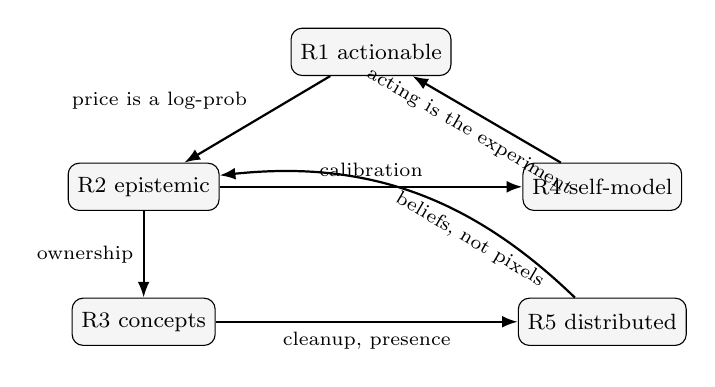
\begin{tikzpicture}[node distance=11mm and 9mm,
  req/.style={draw,rounded corners,minimum width=15mm,minimum height=6mm,font=\footnotesize,fill=gray!8},
  dep/.style={-{Latex[length=2mm]},thick}]
\node[req] (r1) {R1 actionable};
\node[req,below left=of r1] (r2) {R2 epistemic};
\node[req,below right=of r1] (r4) {R4 self-model};
\node[req,below=of r2] (r3) {R3 concepts};
\node[req,below=of r4] (r5) {R5 distributed};
\draw[dep] (r1) -- node[above left,font=\scriptsize]{price is a log-prob} (r2);
\draw[dep] (r2) -- node[above,sloped,font=\scriptsize]{calibration} (r4);
\draw[dep] (r2) -- node[left,font=\scriptsize]{ownership} (r3);
\draw[dep] (r3) -- node[below,font=\scriptsize]{cleanup, presence} (r5);
\draw[dep] (r5) to[bend right=25] node[pos=0.3,below,sloped,font=\scriptsize]{beliefs, not pixels} (r2);
\draw[dep] (r4) -- node[below,sloped,pos=0.55,font=\scriptsize]{acting is the experiment} (r1);
\end{tikzpicture}
\caption{The requirements as a dependency graph. An arrow $A\to B$ reads ``$A$ needs $B$''. Each
arrow corresponds to a measured incident described in \S\ref{sec:coupling}. The cycle is why the set
cannot be satisfied one requirement at a time.}
\label{fig:coupling}
\end{figure}

\section{Related work, by requirement}\label{sec:related}

Rather than survey systems one by one, we organise prior work by the requirements it addresses, and
summarise the result in Table~\ref{tab:related}.

\paragraph{Scene graphs as records} The 3D Scene Graph of Armeni et
al.~\cite{armeni20193dscenegraphstructure} introduced the layered structure of building, rooms,
objects and cameras that later systems adopted. Kimera and its dynamic scene
graphs~\cite{rosinol20203ddynamicscenegraphs,rosinol2021kimeraslamspatialperception} and then
Hydra~\cite{hughes2022hydra,hughes2024foundations} built that structure online from a
metric-semantic reconstruction; ConceptGraphs~\cite{gu2023conceptgraphsopenvocabulary3dscene} and
HOV-SG~\cite{werby24hovsg} opened the vocabulary of labels, and
Khronos~\cite{schmid2024khronosunifiedapproachspatiotemporal} added the temporal dimension. These
are single-pipeline systems in which the graph is an output. The uncertainty of a node, where it is
tracked at all, is stored rather than acted upon, and actions live outside the graph.

\paragraph{Rooms and walls in the loop} S-Graphs~\cite{bavle2022situational,bavleSGraphs20HierarchicalSemantic2025}
comes closest to our second and third requirements at the level of the room: walls and rooms are
factors in a single optimisation, so that the structure of the environment constrains the robot's
pose. The estimator remains a single one, however, and the resulting graph is passive.

\paragraph{Task-driven graphs} Clio~\cite{maggioClioRealtimeTaskDriven2024} clusters the graph
according to the task at hand, and SayPlan~\cite{ranaSayPlanGroundingLarge2023} plans over a scene
graph with a language model. In both, the task is formulated outside the representation and the graph
is what the task reads; in an \asg\ the task is a prior added to the functional the graph already
minimises.

\paragraph{Active SLAM and active inference in robotics} The active-SLAM
survey~\cite{placedSurveyActiveSimultaneous2023} frames exploration as decision-making under
uncertainty and makes the methodological point on which our evaluation rests, namely that an open-loop
recording cannot score a closed-loop policy. Active inference~\cite{friston2010free,friston2015epistemic}
supplies the single functional we use throughout. Its applications in
robotics~\cite{lanillosActiveInferenceRobotics2021,pezzatoMobileManipulationActive2025} have so far
concentrated on control and manipulation rather than on the representation itself.

\paragraph{Our own prior work} CORTEX~\cite{bustos_cortex_2019,proposal-latency-bustos} provides the
distributed working memory on which the present system is built. The concept-first architecture
of~\cite{zapatacornejoConceptGuidedExplorationBuilding2025} showed rooms and doors as cooperating
agents, and the IWAI abstract~\cite{bustos2026active} introduced the actionable graph with a
Fisher-information selector. The requirements, their coupling, the pricing and the self-model are new
to this paper.

\paragraph{The term} ``Active scene graph'' also appears in computer vision, where it denotes active
learning for image scene-graph generators. \todo{search and cite one representative; disambiguate in
a footnote}. We use the phrase in the control sense: a graph that acts.

\begin{table}[t]
\centering\small
\caption{Systems against requirements. $\bullet$ met, $\circ$ partial, blank not addressed. \todo{verify each cell against the cited paper before submission.}}
\label{tab:related}
\setlength{\tabcolsep}{4pt}
\begin{tabular}{lccccc}
\toprule
System & R1 & R2 & R3 & R4 & R5 \\
\midrule
3D Scene Graph~\cite{armeni20193dscenegraphstructure} & & & & & \\
Kimera, Hydra~\cite{rosinol20203ddynamicscenegraphs,hughes2022hydra} & & $\circ$ & & & $\circ$ \\
S-Graphs~\cite{bavle2022situational} & & $\circ$ & $\circ$ & & \\
ConceptGraphs~\cite{gu2023conceptgraphsopenvocabulary3dscene} & & & & & \\
Clio~\cite{maggioClioRealtimeTaskDriven2024} & $\circ$ & & & & $\circ$ \\
SayPlan~\cite{ranaSayPlanGroundingLarge2023} & $\circ$ & & & & \\
Concept-first rooms~\cite{zapatacornejoConceptGuidedExplorationBuilding2025} & & $\circ$ & $\bullet$ & & $\bullet$ \\
This work & $\bullet$ & $\bullet$ & $\bullet$ & $\bullet$ & $\bullet$ \\
\bottomrule
\end{tabular}
\end{table}

\section{Definition: the Active Scene Graph}\label{sec:def}

Fig.~\ref{fig:viewer} shows a live \asg\ as its viewer agent draws it, with the graph's strata
pulled apart vertically so that the structure is visible: the robot at the bottom, the room with
its walls and doors above it, the object instances above that, their parts, and at the top the
meta-concepts that group instances into a kitchen or a dining set. Every element in the figure is a
node with a posterior behind it, and every line is a typed edge.

\begin{figure}[t]
\centering
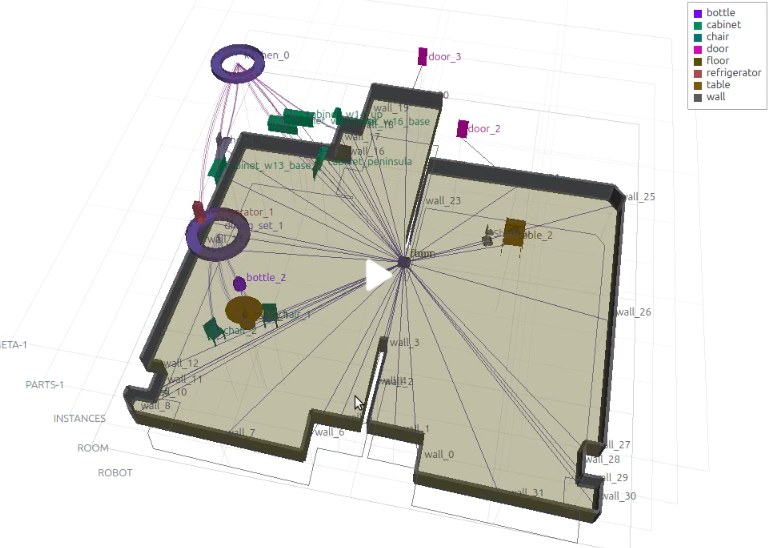
\includegraphics[width=\columnwidth]{fig/asg_viewer}
\caption{A live Active Scene Graph, captured from the fleet's viewer agent during a run in the
simulated apartment. The strata (robot, room, instances, parts, meta-concepts) are separated
vertically. The room is a polygon of walls with three doors; the instances are tables, chairs,
cabinets, a refrigerator and a bottle, each drawn from its own belief; the two rings at the top are
meta-concepts, a kitchen and a dining set, that group instances by their spatial relations. Lines
are the graph's edges, most of them \texttt{RT} transforms from the room frame.}
\label{fig:viewer}
\end{figure}

\subsection{Nodes are concepts}

A node $n$ is a tuple $(c,\,\mu_n,\,\Sigma_n,\,\Pi_n,\,\ell_n,\,a_n)$ consisting of a class $c$, a
posterior mean and covariance over the parameters of that class, a precision $\Pi_n$ attached to the
observation channel that feeds the node, a log-odds of existence $\ell_n$, and the identity $a_n$ of
the agent that owns it. The parameters depend on the class: a room is a polygon of corners together
with a pose, a table is a box with a height, a bottle is a cylinder, and a door is a hinge line with a
width and an opening angle. Each class comes with a generative model of what the sensors return given
the parameters, and we write these models as signed distance fields so that the likelihood is
differentiable in the parameters: the polygon of a room evaluated against LiDAR returns, a table as a
smooth log-sum-exp box top on four cylindrical legs, a bottle as a cylinder. The same distance field
serves both for fitting the belief and, projected through the camera model, for computing the
expected information gain of a candidate view.

\subsection{Edges are typed and timestamped}

Geometry is carried by \texttt{RT} edges that hold a rigid transform together with a timestamp and a
covariance, so that a consumer can extrapolate a lagging frame using the producer's twist and can
weight a transform by how far it is trusted. Three further edge types carry the active part of the
graph. A \texttt{has\_intention} edge links a concept node to the affordance nodes it publishes; an
\texttt{executing} edge links the controller's own node to the affordance it is currently carrying
out; and a \texttt{proto} self-edge marks a node whose identity is not yet resolved, such as a room the
robot has just entered through a door and has not yet recognised either as new or as one it has
visited before.

\subsection{Agents are owners}

Every node is created, updated and removed by exactly one agent, whose identity is stored on the
node. That agent is the process running the class's generative model, and it is a peer in a
distributed graph rather than a stage in a pipeline: it starts, declares which peers it needs, serves
while they are present, and cleans up its own nodes when it stops.

\subsection{The lifecycle contract is the operational semantics}

What an agent may do to the shared graph is fixed by a contract with five stages. Under
\emph{create}, a node is born only from a tracker that has associated several frames, never from a
single detection. Under \emph{update}, a frame may move geometry only if its frame is resolvable, its
subject is centred in the image, and the robot is still enough that the variance induced by its own
motion does not dominate. Under \emph{remove}, the only evidence for removal is that the object was
predicted visible and was absent, weighted by \pdet\ and requiring a clear line of sight through the
walls; occlusion holds the belief where it is, and miss counters are not permitted. Under
\emph{history}, no agent may use a constant process noise, since the volatility of a concept is
something to be inferred from its own past. Under \emph{ownership}, the identity stored on the node
must match the agent that writes it. A conformance audit (\S\ref{sec:eval:r3}) checks every agent
against every stage.

\section{One objective, two regimes}\label{sec:efe}

Every quantity the controller compares is a log-probability, and there is one functional, the
expected free energy of a policy $\pi$,
\begin{equation}
\efe(\pi) = \underbrace{-\,\mathbb{E}_{q}\big[\log C(o_\pi)\big]}_{\text{pragmatic}}
\;-\;\underbrace{\mathbb{E}_{q}\big[H(s) - H(s\,|\,o_\pi)\big]}_{\text{epistemic}},
\label{eq:efe}
\end{equation}
in which the task layer differs from the representational layer only through the prior preference
$C$.

With a flat $C$ only the epistemic term survives, and this is the fleet's default: move so as to
represent, and stay aligned with the world. It is the always-on layer, and it is what an \asg\ does
when nobody has asked it for anything. With a sharp $C$ over a goal state, for instance that the
robot be in room B, the pragmatic term dominates, and an epistemic offer that lies off the route is
taken exactly when its information gain exceeds the pragmatic loss of the detour, measured in the same
units. The familiar instruction to take a detour only if it does not perturb the goal too much becomes
this inequality rather than a rule.

\subsection{The price table}

Table~\ref{tab:price} lists each term the controller sums, the agent that produces it, and the
hand-set constant that the term replaces. Where a constant survives in the present code, the table
says so and indicates what should replace it.

\begin{table*}[t]
\centering\small
\caption{Every term the controller compares, in \nats. The last column names the constant each term retires, or the constant that remains.}
\label{tab:price}
\begin{tabular}{P{2.6cm}P{5.6cm}P{2.6cm}P{5.6cm}}
\toprule
\textbf{Term} & \textbf{Price} & \textbf{Producer} & \textbf{Retires / remains} \\
\midrule
Epistemic value of an offer & $\pdet\cdot\Delta H$, with $\Delta H = H(\Sigma) - H(\Sigma^\star)$ under the concept's own model & each concept, from its own $\Sigma$ & per-class gain scales. One survives (\texttt{aff\_room\_gain\_scale}=0.35); if a scale is needed the units are not homogenised, so it must go. \\
Precondition & $\log p(\text{precondition})$; a door open with $p=0.3$ costs $-1.2$ \nats; $p=0$ is not an offer & pragmatic-affordance producer & on/off gating (presence of a precondition rather than its probability) \\
Navigation cost & expected growth of self-entropy along the path, $\tfrac12\log\det(\Sigma_{\mathrm{pose}}+Q(\text{path})) - \tfrac12\log\det\Sigma_{\mathrm{pose}}$, with $Q$ from the self-model's calibrated motion noise (R4), plus $\log(1-p_{\mathrm{coll}})$ along the path, plus delay against $C$ & controller, from the robot concept & $\lambda\cdot d_{\mathrm{nav}}$ with $\lambda = 0.2$ \nats/m: a constant that should be a function of the calibrated $Q$. Still in the code; kept as an A/B flag. \\
Commitment & a hysteresis margin: switch only if $\efe(\text{incumbent}) - \efe(\text{challenger}) > m$ & controller & $m = 0.5$ \nats\ remains. Derivable as the expected loss of the half-executed policy; not done. \\
Existence & log-odds; absence weighted by \pdet; occlusion adds 0 & shared existence module & miss counters, debounce timers \\
Publication gate & the adequacy gap between the posterior $\Sigma$ and $\Sigma^\star$, in \nats & each concept & tuned publish bounds \\
\bottomrule
\end{tabular}
\end{table*}

Two properties make this table work across a fleet of independent agents. Because each producer
computes $\Delta H$ from its own $\Sigma$, the units are homogeneous by construction and no
cross-class scale is required. And because the executor never learns what a door is, the affordance's
kind being a label used for logging rather than a dispatch key, a new concept can add offers without
any change to the controller.

\subsection{Interruption is re-scoring}

Selection, horizon and interruption are one and the same comparison. The incumbent, if there is one,
is the offer under an \texttt{executing} edge; the challenger is the minimiser of $\efe$ over
everything currently offered; and a switch fires when the incumbent's price exceeds the challenger's
by the commitment margin. Since producers decay their epistemic gain as their $\Sigma$ shrinks during
execution, an incumbent that is nearly resolved loses naturally to a fresh challenger, and the
interruption emerges from the value dynamics without a rule saying when to stop. The margin itself is
the one constant that remains in this part of the system.

\section{The robot as a concept}\label{sec:self}

The robot is a node in the graph with a frame tree beneath it: the base, the sensor mounts, and the
rigid transforms between them. What distinguishes it from a table is only that its parameters are also
parameters of the measurement model of everything else, and the fourth requirement says that these
parameters are beliefs, updated online like any other.

\paragraph{What is learnable} On the platforms we use, low-level velocity loops hide the dynamics, so
what remains to be learned is kinematic: the scale and rotation gain of the wheel odometry, and the
extrinsics of each camera relative to the LiDAR. Dead reckoning cannot calibrate itself, since from
inside the odometry an error and a true motion look the same. What breaks the symmetry is an absolute
reference, and the localiser already has one in the room polygon against which the distance field
anchors the posterior. Its error does not grow with distance travelled, which makes it an independent
witness of true motion.

\paragraph{The free teacher} The localiser's own correction is the teacher. Every cycle it predicts
the pose from the motion model and corrects it from the map, and the correction is the residual the
calibration must explain. A batch estimator over episodes solves jointly for the kinematic and
extrinsic parameters that minimise these corrections, under the same free energy the localiser
minimises over states. The parameters are separable only if each loads on a different component of
the correction through a different covariate. This is why the rotation gain, which loads on heading
through angular speed, and the translational scale, which loads on position through linear speed, can
be told apart, and it is also why the height of a camera mount cannot be separated from the height of
the ceiling it observes (\S\ref{sec:eval:r4}).

\paragraph{Why there is no calibration affordance} It would be natural to publish an offer that
reads ``calibrate yourself''. We do not, for the reason expressed by the arrow from R4 to R1 in
Fig.~\ref{fig:coupling}: the free energy of the self-model does not fall because the robot computed
harder, but because it moved and the map disagreed with the prediction. We measured this directly.
Across an injected scale error ranging from 0 to 10\%, the solver's iteration count stayed flat between
13.3 and 13.9, while the correction load $|\text{estimated} - \text{predicted}|$ tracked the error
faithfully. Acting is the experiment, and the ordinary offers generate all the evidence the self-model
needs.

\paragraph{Downward coupling} A correction to a parameter propagates into every belief that was fitted
through it, so that corrected extrinsics re-price every offer that depends on where a camera points.
Our rule is that this propagation may only loosen a belief and never tighten it, and that the slower
convergence which results is the correct behaviour. This mechanism is specified but not yet built
(Table~\ref{tab:ledger}).

\section{Architecture}\label{sec:arch}

The third and fifth requirements are met by an architecture with four parts.

\paragraph{The graph} A conflict-free replicated graph, inherited from
CORTEX~\cite{bustos_cortex_2019,proposal-latency-bustos}, is held in full on every agent's machine.
Writes merge without a coordinator, signals fire on every peer when a node or edge changes, and every
attribute is typed at compile time.

\paragraph{The media plane} Sensor streams do not enter the graph. A producer advertises, on the
sensor's node, a descriptor naming a topic on a dedicated DDS domain, and consumers subscribe to that
topic without copying. The graph carries beliefs and descriptors; the plane carries pixels and
points. This is the arrow from R5 to R2 in Fig.~\ref{fig:coupling}: bandwidth is bounded because the
representation is parametric.

\paragraph{The presence protocol} An agent declares the peers it requires, begins serving only once
they are present, and degrades when one of them leaves. Degradation is debounced, so that a transient
flap does not trigger cleanup. We modelled the protocol in TLA+ and checked it exhaustively, verifying
eight safety invariants and four liveness properties over \num{65536} states for a three-agent
instance. The model abstracts away heartbeat timing, and it is worth recording that the failure which
later stopped the fleet was precisely a timing failure, the undebounced flap. A proof about a
specification and a specification that survives contact with the world are different achievements,
and the protocol now has both.

\paragraph{The affordance protocol} A producer publishes an offer with a target and an epoch. The
controller claims it by writing an \texttt{executing} edge that it owns, carrying the epoch and the
pose it is actually driving towards. The producer then measures progress against the consumer's
stated target rather than against its own latest proposal, and a mismatch of epochs is detectable by
either side. An earlier version of this protocol returned only a boolean, and the TLA+ model of that
version reproduces its failure in a four-state counterexample; with the claim carried on the edge, the
model is clean at three times the bound (\num{22815} states). The invariant behind the fix is general:
no party may judge another by a quantity the other cannot observe.

\begin{table}[t]
\centering\small
\caption{Ledger: what is designed (D), implemented (I) and evaluated (E).}
\label{tab:ledger}
\begin{tabular}{P{5.2cm}ccc}
\toprule
\textbf{Mechanism} & D & I & E \\
\midrule
Concept nodes with $(\mu,\Sigma,\Pi,\ell)$, SDF likelihoods & $\bullet$ & $\bullet$ & $\bullet$ \\
Epistemic offers priced by $\pdet\cdot\Delta H$ & $\bullet$ & $\bullet$ & $\bullet$ \\
Pragmatic offers (door approach / open / cross) & $\bullet$ & $\bullet$ & \\
$\log p(\text{precondition})$ instead of on/off & $\bullet$ & & \\
Task prior $C$ in the controller & $\bullet$ & & \\
Navigation cost from calibrated $Q$ (replacing $\lambda$) & $\bullet$ & & \\
Existence as \pdet-weighted log-odds & $\bullet$ & $\bullet$ & $\bullet^{a}$ \\
Room structural adoption judge & $\bullet$ & $\bullet$ & $\bullet$ \\
Lifecycle contract and conformance audit & $\bullet$ & $\bullet$ & $\bullet$ \\
Self-model: wheel covariance, preintegration & $\bullet$ & $\bullet$ & $\bullet$ \\
Self-model: closed-loop camera extrinsics & $\bullet$ & $\bullet$ & $\bullet$ \\
Self-model: batch estimator over episodes & $\bullet$ & $\bullet$ & $\bullet$ \\
Downward coupling (loosen-only propagation) & $\bullet$ & & \\
Proto-room: navigate while the layout is estimated & $\bullet$ & $\bullet^{b}$ & \\
Presence protocol (TLA+) & $\bullet$ & $\bullet$ & $\bullet$ \\
Affordance claim protocol (TLA+) & $\bullet$ & $\bullet$ & $\bullet$ \\
Media plane, zero-copy & $\bullet$ & $\bullet$ & $\bullet$ \\
Bounded CRDT history & & & \\
\bottomrule
\multicolumn{4}{l}{\footnotesize $^{a}$ evaluated for tables, doors, cabinets, refrigerators; not yet for bottles.}\\
\multicolumn{4}{l}{\footnotesize $^{b}$ built and compiled; first live test pending.}
\end{tabular}
\end{table}

\section{Evaluation}\label{sec:eval}

\subsection{Premise}

The evaluation of an active system has a constraint that a passive one does not. A dataset is an
open-loop recording, and under \eqref{eq:efe} the observations a robot receives depend on the actions
it chooses, so replaying a fixed sequence scores one policy on data that a different policy
generated. The comparison that carries information is therefore policy against policy inside a single
closed loop, with body, sensors, noise, timing and environment held fixed and only the decision rule
varied~\cite{placedSurveyActiveSimultaneous2023}. Our comparators are the heuristics that each
mechanism replaced. These were written by people who wanted them to work, tuned until they did, and
shipped in a running fleet, which makes them demanding baselines rather than convenient ones.

The platforms are a Webots simulation of a two-room apartment running the same component code as
the robots; Shadow, a differential-drive robot with a 360$^\circ$ LiDAR, a stereo camera and a
panoramic camera; and P3Bot, an omnidirectional mobile manipulator carrying two Kinova Gen3 arms and
its own LiDAR. The fleet of agents is identical on all three, and only the robot concept differs:
the base kinematics, the sensor mounts and the arms are properties of that one node.

\subsection{R2: the uncertainty is consumed}\label{sec:eval:r2}

\paragraph{Calibrated corners on a physical robot} The room concept declares a corner publishable
when its posterior $\sigma$ falls below a bound. On the physical robot, measured against a surveyed
room, a corner declared publishable has a median true error of \SI{2.0}{cm} and lies within its
declared \SI{6}{cm} in \SI{86}{\percent} of cases, whereas a corner that is withheld has a median
error of \SI{3.6}{cm} and lies within the bound in \SI{64}{\percent} of cases. The declared
uncertainty separates good corners from bad ones, which is what the requirement asks of it. The full
study appears in a companion paper and we do not repeat its figures here.

\paragraph{Room shape from an epistemic explorer} On \num{50} synthetic rooms with adversarial spurs
and alcoves, replacing a coverage heuristic by the information-gain explorer raised the median layout
IoU from \num{0.947} to \num{0.954}, and lifted the worst room, an L shape, from \num{0.812} to
\num{0.944}.

\paragraph{A null result, and its cause} On \num{594} real annotated floor plans, with runs paired
by room, the same explorer against the same heuristic gives a mean IoU difference of $-0.0007$ with a
95\% confidence interval of $[-0.0019,\,+0.0004]$; the heuristic wins 263 rooms, the explorer 251, and
69 are tied. On this corpus the epistemic term buys nothing, and the reason is instructive. Every room
in both arms ran to the 900-frame budget (594 of 594 and 593 of 594), so the final map was measured at
saturation, a point at which any reasonable policy has already seen every wall. An objective cannot
be graded on an endpoint that its own budget has saturated, and the number which predicts the null,
the 594 of 594 at the cap, was available before the run began. What the experiments support is that
the uncertainty is consumed: it gates publication and the explorer reads it. What they do not show is
that the epistemic term buys accuracy or speed over a simple heuristic at the scale of a single room.
Tighter budgets and multi-room environments are where a difference would have to appear, and those
settings remain to be tested.

\subsection{R1: one executor, offers from any concept}\label{sec:eval:r1}

The affordance claim protocol is evaluated both formally (\S\ref{sec:arch}) and in operation. Once the
epoch and the owned edge were introduced, the refusal loop in which a re-armed offer appeared new to
the controller on every cycle fell from \SI{47}{\percent} of decisions to \SI{7}{\percent}, and the
stream of protocol events that producers had been generating to reconcile their view of the target,
some \num{12} per second, ceased entirely. The door offers to approach, open and cross are built and
compile against the same executor with no door-specific code in the controller, and their first live
run is pending. The task-level experiment the design calls for, with one room, one door and one live
epistemic offer while the controller logs the decomposition of \efe\ for each candidate at each
decision, is the first item of future work.

\subsection{R3: the lifecycle contract in practice}\label{sec:eval:r3}

A conformance audit checks each of eight concept agents against the five stages of the contract and
three subsidiary conditions: the admissibility of a frame, the weighting of absence by \pdet, and line
of sight through walls. At the audit of 2026-07-31, five agents conformed on every column, two
conformed except for an attributable history, and one, the inherited human concept, met only the
ownership stage and is scheduled for rewrite. The clearest effect of the contract is on phantoms.
Bringing the bottle concept under the create stage, so that a node is born from a tracker rather than
from a single frame, reduced phantom births on a fixed tour from \num{130} to \num{1}. Ownership is
enforced at startup: an agent refuses to start if the node it would own already carries another
agent's identity.

\subsection{R4: the self-model learns from its own corrections}\label{sec:eval:r4}

\paragraph{Extrinsic attribution} On a single recorded tour we inject a $1^\circ$ yaw error in turn
into the panoramic camera, the stereo camera and the LiDAR, and observe what the closed-loop extrinsic
estimator recovers. The stereo camera's yaw is recovered at $0.984 \pm 0.018$ of the injected value
and the panoramic camera's at $0.454 \pm 0.175$, while an error injected into the LiDAR appears in
both cameras and not in their closure ($-0.018$), which identifies the misaligned device. The
asymmetry between the two cameras is itself a finding. On a panorama a yaw is a constant pixel shift
and cannot be told from a corner's own offset, whereas on a pinhole camera the shift grows towards the
edge of the field as $\sec^2\theta$, so that a single corner seen across the image separates yaw from
offset by itself. The uniformity that lets the panorama separate pitch from height is exactly what
costs it yaw, and the two cameras turn out to be complementary.

\paragraph{A bias the precision could not see} The same estimator found a boresight error of
$+0.814^\circ$ in the stereo camera which the corner channel had been absorbing as a smaller declared
$\sigma$ rather than a larger error. Applying that correction is what allowed the corner calibration
reported above to hold, and it is the chain from R1 through R2 to R4 observed in a measurement.

\paragraph{What we do not publish} The estimator also produces a mount height and a pitch for each
camera, and we leave both unpublished. Floor corners and ceiling corners disagree by \SI{116}{mm}
about the height of one mount while agreeing on its yaw to $0.0006^\circ$, which tells us that the
height channel is measuring the ceiling constant of the room rather than the mount. A parameter is
learnable only if it loads on a covariate nothing else loads on, and here it does not.

\paragraph{Odometry} Wheel-odometry covariance is injected each cycle as a function of speed. The
rotational variance had to be raised by a factor of \num{580} above the vendor's constant before the
localiser's normalised innovation became consistent, and a zero-velocity update whose $\sigma$ had
been measured on one robot proved 5.9 to 7.3 times too tight on the other. This is why the robot
concept, rather than a shared constant, owns these quantities.

\subsection{R5: latency and membership}\label{sec:eval:r5}

Table~\ref{tab:lag} gives the age of each stream at the consumer before and after two changes to the
producers: a drift-free trigger aligned to the sensor's acquisition grid, and duplicate suppression.
The floor is set by the source rather than the transport, since the data is already \SI{17}{ms}
(LiDAR) to \SI{27}{ms} (RGB-D) old when the simulator hands it over, and the plane adds under
\SI{10}{ms} above that. The LiDAR stream runs at \SI{20}{Hz}, which is the rate of its source.

\begin{table}[t]
\centering\small
\caption{Stream age at the consumer, ms, measured on 2026-09-10.}
\label{tab:lag}
\begin{tabular}{lS[table-format=2.1]S[table-format=2.1]}
\toprule
Stream & {before} & {after} \\
\midrule
LiDAR (Helios)   & 35.2 & 8.8 \\
LiDAR (Bpearl)   & {--} & 10.0 \\
Panoramic RGB    & 50.2 & 11.1 \\
Stereo RGB-D     & 36.0 & 9.0 \\
\bottomrule
\end{tabular}
\end{table}

Agents are started and stopped in arbitrary order in every session. A graceful stop removes the
agent's owned nodes, and a restart re-adopts orphaned ones under the ownership rule. The one defect
we know of in this layer is described in \S\ref{sec:limits}.

\subsection{Localisation and object beliefs against ground truth}

Two further numbers from the same fleet allow the beliefs the graph carries to be judged as beliefs.
Against simulator ground truth over 4 runs and \num{5468} poses, the room-anchored localiser has a
median position error of \SI{72}{mm}, \SI{145}{mm} at the 90th percentile and $0.8^\circ$ in
heading, running at \SI{19.1}{Hz}. For the bottle concept, against ground truth over \num{2173}
rows, the position RMSE is \SI{13.6}{mm} with a median normalised estimation error squared of
\num{0.46}. The covariances are consistent with the errors, which is the precondition for pricing
offers from them at all.

\section{Limitations}\label{sec:limits}

Several parts of the system are further along in design than in evidence, and we set them out here.
The epistemic term has not been shown to outperform a heuristic at the scale of a single room, for
the reason given in \S\ref{sec:eval:r2}, and the multi-room, budget-limited experiment in which a
difference could appear has not yet been run. The task-level functional with a sharp $C$ is designed
but not implemented, so the evaluation of the first requirement concerns the protocol rather than a
task. Two constants remain in the controller, the commitment margin and the navigation weight
$\lambda$, until the latter is replaced by the calibrated $Q$; both are named in
Table~\ref{tab:price}. The history of the replicated graph is unbounded, since the per-node version
vector grows with every write, and on long sessions the merge cost reached a full processor core at
\num{318000} entries; until the history is bounded, the fifth requirement holds for the length of a
session. The detectability envelope \pdet\ is fitted in simulation for the classes reported here, and
its calibration on real images is the subject of a separate paper. The self-model's translational
scale inherits the map's error, so a room polygon two percent too large hands two percent to the
scale; rotation is immune to this, while translation is only as good as the survey. Finally, the
proto-room mechanism that lets the robot navigate while a new room is still being estimated is built
and compiled but awaits its first live run.

\section{Conclusion}

An Active Scene Graph is a scene graph whose nodes are beliefs, whose beliefs publish what would
reduce them, whose robot is one of its own beliefs, and whose controller prices everything in a
single currency. We have argued that the five requirements this entails are coupled, presented a
system that meets them together, and reported what its evaluation supports and where the evidence
still has to be gathered. The next version of this preprint will add the task-layer experiment on the
physical robot and the multi-room setting in which an epistemic explorer can be expected to make a
difference.

\section*{Acknowledgements}
\todo{funding lines}

\balance
\bibliographystyle{IEEEtran}
\bibliography{refs}

\end{document}
